\scanpage{4}
par des autom \uline{unimodulaires}, \deleted{\unsure{ils sont|il est}} On
comprendra mieux par la suite la nature
exacte de cette restriction (en étudiant
le pt de vue projectif)\,; disons pour
l'instant qu'on verra qu'il revient au
$=$ d'exiger $\sigma_a$ (l'un ou tous, \unsure{cel|cela}
revient au $=$ puisqu'ils sont conjugués)
est une réflexion -- i.e. laisse invariant
une droite. On verra aussi que cette
restriction est automatiquement satisfaite
\uline{sauf} dans le cas d'un polygône régulier
à $2p$ côtés en car $p$ ($p$ nb premier
impair) -- p.ex. l'hexagone en car. 3.

% slanted
\margin{\uline{Devrait remonter}}
NB \quad On fera attention que dans la définition
du polygône général, on avait défini
les côtés comme des \uline{droites} de $E$
-- on a une application \deleted{surjective} de
l'ens des côtés combinatoires \uline{sur} l'ens
des côtés géométriques. On dira
que le polygône est \uline{propre} si pour un sommet
$s\in S$ et un côté combinatoire $\{s',s''\}$, $s$
\figure{\begin{tikzpicture}[x=1cm,y=1cm]
\draw (0,0)--(.87,.28);
\end{tikzpicture}}
\figure{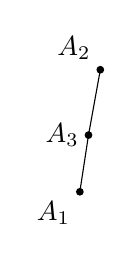
\begin{tikzpicture}[x=1cm,y=1cm]
\draw (.02,0)--(.13,.72)--(.28,1.55);
\fill (.02,0) circle (1.4pt) node[below left] {$A_1$};
\fill (.13,.72) circle (1.4pt) node[left] {$A_3$};
\fill (.28,1.55) circle (1.4pt) node[above left] {$A_2$};
\end{tikzpicture}}
\figure{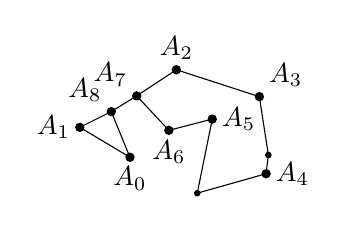
\begin{tikzpicture}[x=.95cm,y=.95cm]
\coordinate (a1) at (0,1.04); \coordinate (a8) at (.42,1.25);
\coordinate (a7) at (.76,1.46); \coordinate (a2) at (1.29,1.81);
\coordinate (a3) at (2.40,1.45); \coordinate (a4) at (2.49,.42);
\coordinate (a5) at (1.77,1.15); \coordinate (a6) at (1.19,1.00);
\coordinate (a0) at (.67,.64);
\draw (a0)--(a1)--(a8)--(a7)--(a2)--(a3)--(2.52,.67)--(a4)--(1.57,.16)--(a5)--(a6)--(a7);
\draw (a8)--(a0);
\foreach \p/\t/\d in {a0/0/below,a1/1/left,a2/2/above,a3/3/above right,a4/4/right,a5/5/right,a6/6/below,a7/7/above left,a8/8/above left}
{\fill (\p) circle (1.7pt) node[\d] {$A_{\t}$};}
\fill (1.57,.16) circle (1.2pt); \fill (2.52,.67) circle (1.2pt);
\end{tikzpicture}}
% archive sheet number: 3

